% !TeX spellcheck = en_US
% !TEX root = ../thesis-example.tex
%

\begingroup
\let\cleardoublepage\clearpage

\chapter{Unitys' Monobehaviour Loop}
\label{app:engineloop}

The behavior of a Unity-initiated object is outlined by the following 
flowchart in \ref{fig:appendix:monoflow}, taken from Unitys' manual.

\begin{figure}[htb]
	\centering
	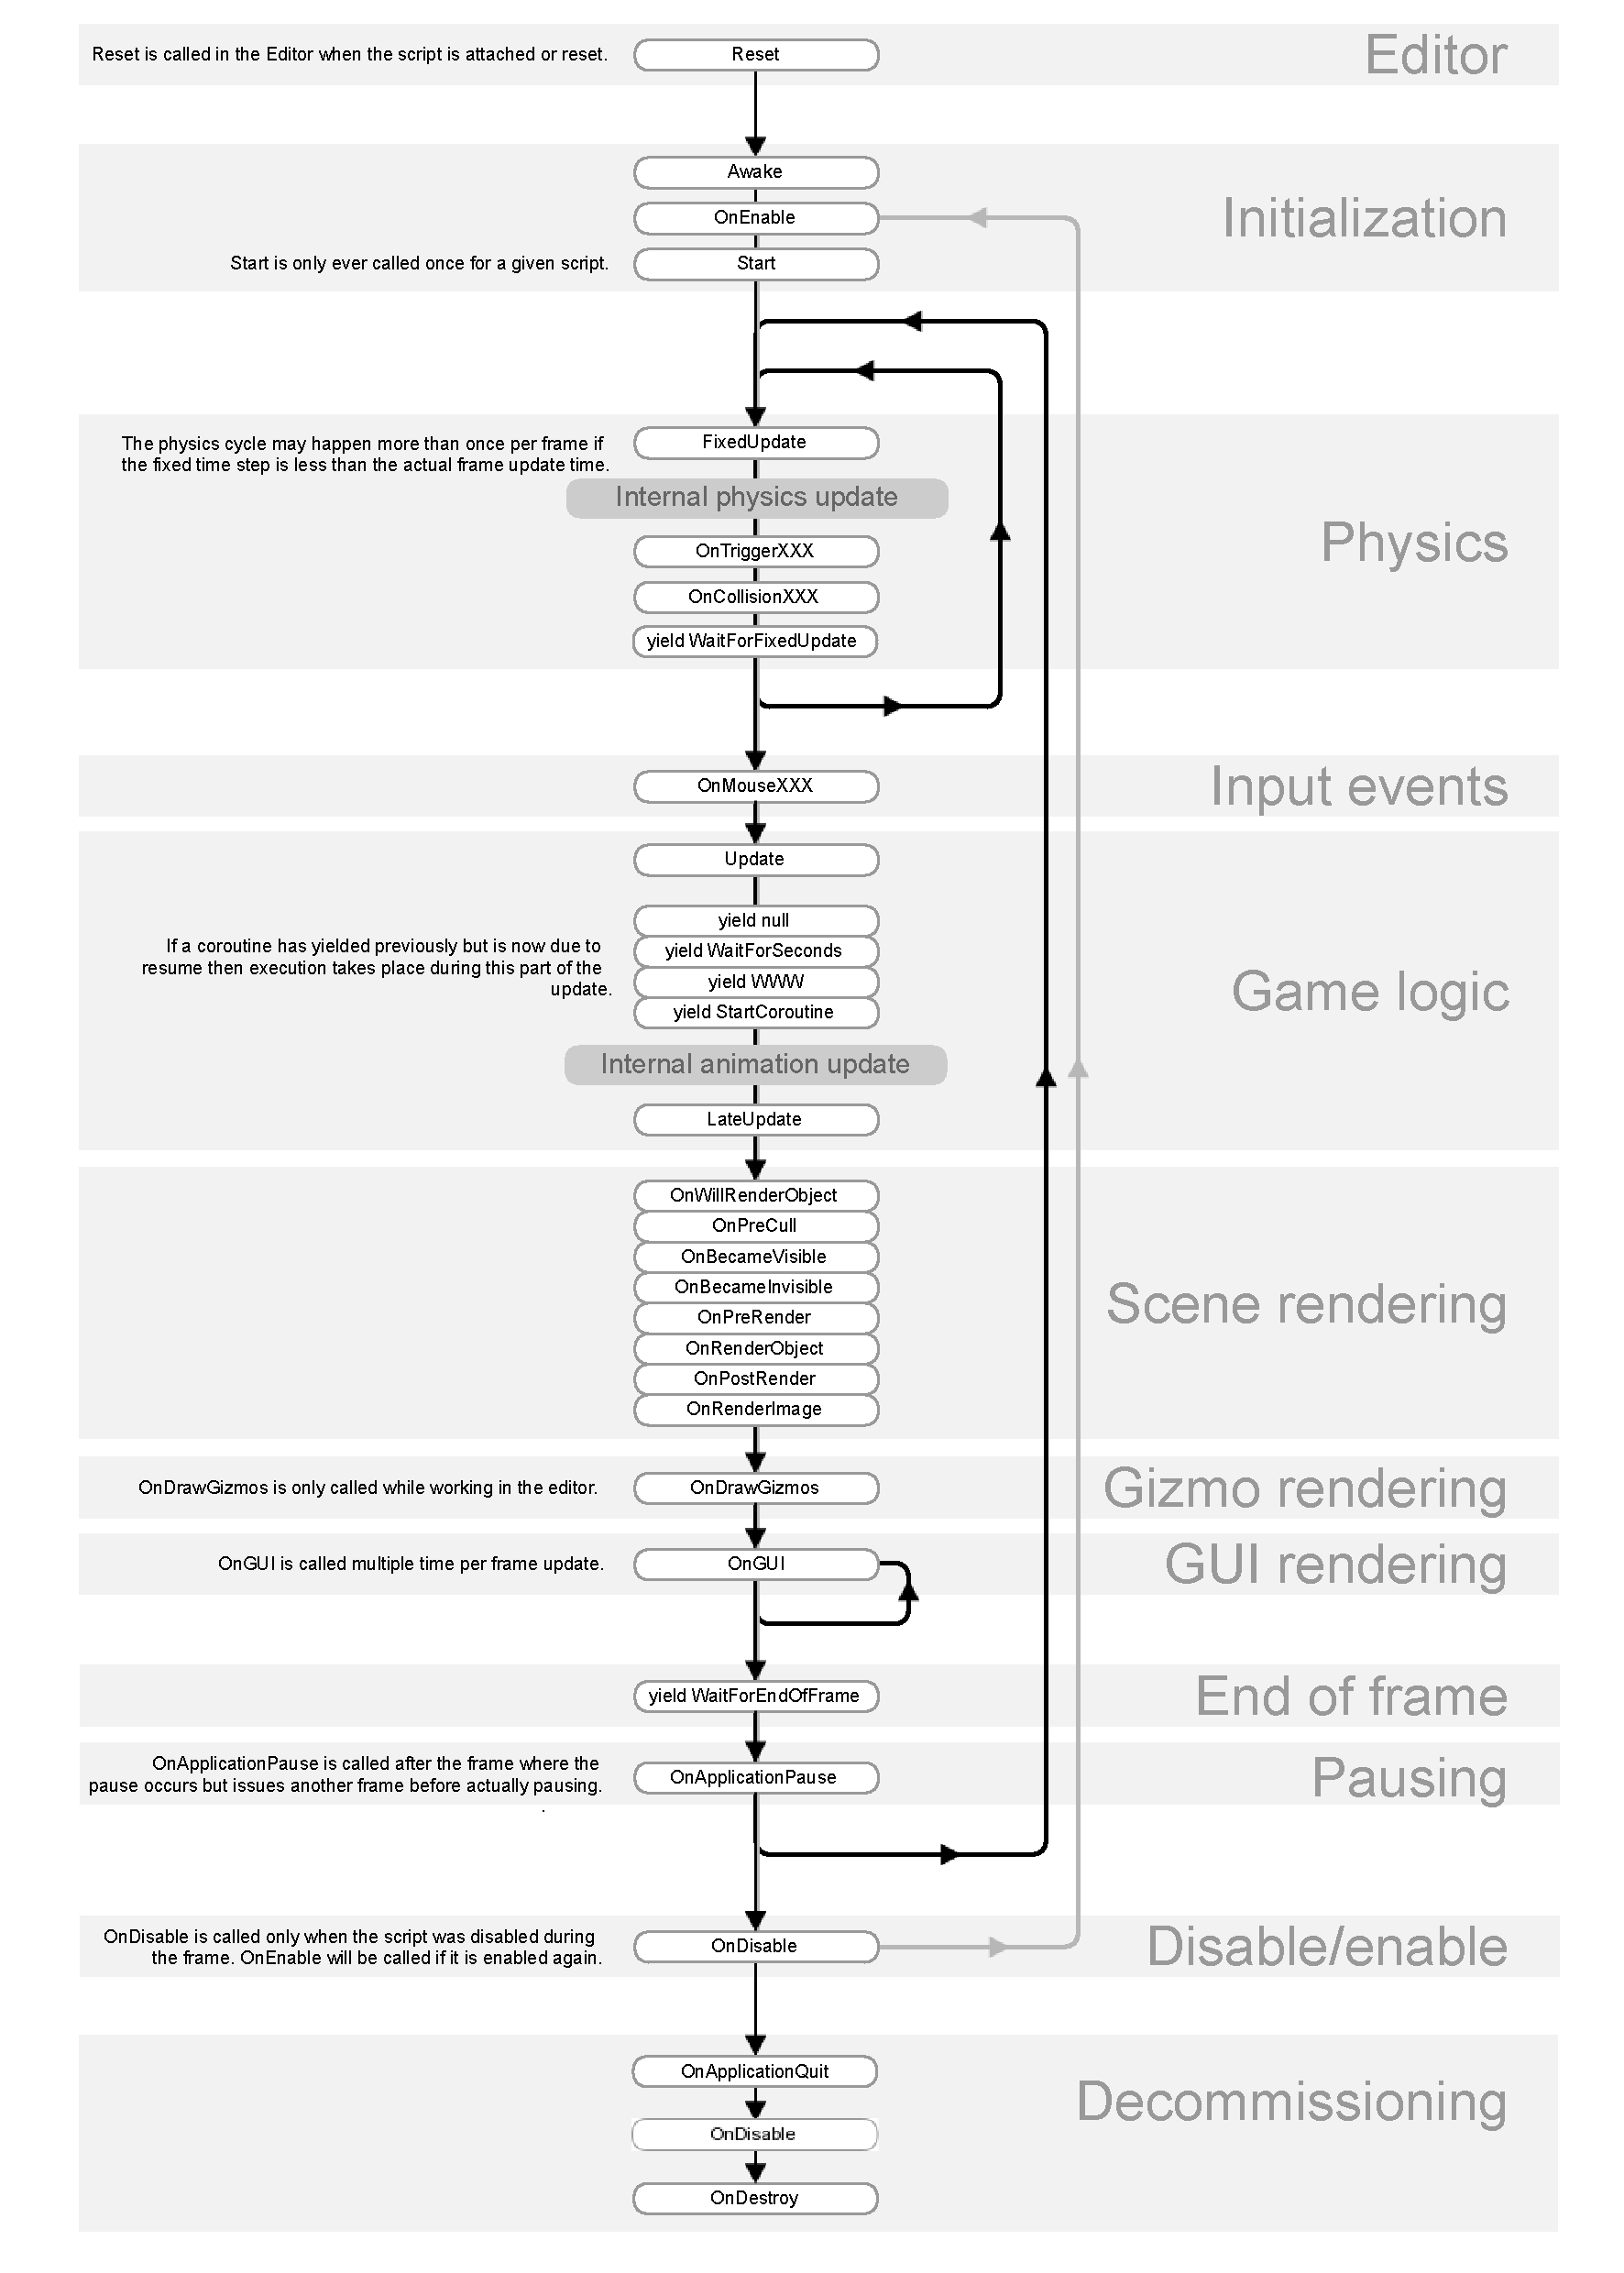
\includegraphics[width=0.85\textwidth]{_external/media/monobehaviour_flowchart2.pdf}
	\caption{Monobehaviour Flowchart}
	\label{fig:appendix:monoflow}
\end{figure}


\chapter{Simple Green Screen Setup}
\label{app:lightningsetup}

Building a green screen set is no easy task and takes a lot of careful 
consideration in light setup, background coloring and material used on set. 
\newline
Figure \ref{fig:appendix:gs-setup} shows a very simple and low-cost green 
screen setup after Foster et al. \cite{foster:greenscreen:2010}

\begin{figure}[htb]
	\centering
	\includegraphics[width=\textwidth]{gfx/appendix/gs-setup.png}
	\caption{Basic green screen setup}
	\label{fig:appendix:gs-setup}
\end{figure}

\chapter{Double Access Ring Buffer Implementation}
\label{app:darbi}

The implementation for an efficient double access ring buffer can seen in the 
following listing:

\begin{lstlisting}[language={[Sharp]C}]
class DoubleAccessRingBuffer<T> {
	public int bufferSize;
	private List<T> buffers;
	private int index;
	
	public DelayedRingBuffer(int bufferSize) {
		this.bufferSize = bufferSize;
		index = 0;
		buffers = new List<long>();
		RebuildBuffers();
	}
		
	public T[] Next(T writeTo, T display) {
		index %= buffers.Count;
		T writeTo = buffers[index];
		T display = buffers[(index + 1) % buffers.Count];
		if(bufferSize != buffers.Count) {
			RebuildBuffers();
		}
		index++;
		return new T[]{writeTo, display};
	}
	
	void RebuildBuffers() {
		buffers.RemoveAll(_ => true);
		for(int i = 0; i < bufferSize; i++) {
			buffers.Add(new T());
		}
	}
}
\end{lstlisting}

\endgroup